% Условная компиляция для самостоятельной работы
\ifdefined\mainfile
    % Если это часть основного файла, не добавляем начало и конец документа
\else
    \documentclass[12pt, a4paper]{report}
    \usepackage{/Users/vladbelousov/Desktop/Semestr_4-FP-NSU/Настройка/library}
    \usepackage[utf8]{inputenc} % Подключение поддержки UTF-8
    \begin{document}
\fi

%%-------------------------------%%

Пусть \(\displaystyle  0 < kz < \frac{\pi}{4}   \Rightarrow 0 < \sin (kz ) < \cos (kz ) < 1 \) 

\begin{center}
    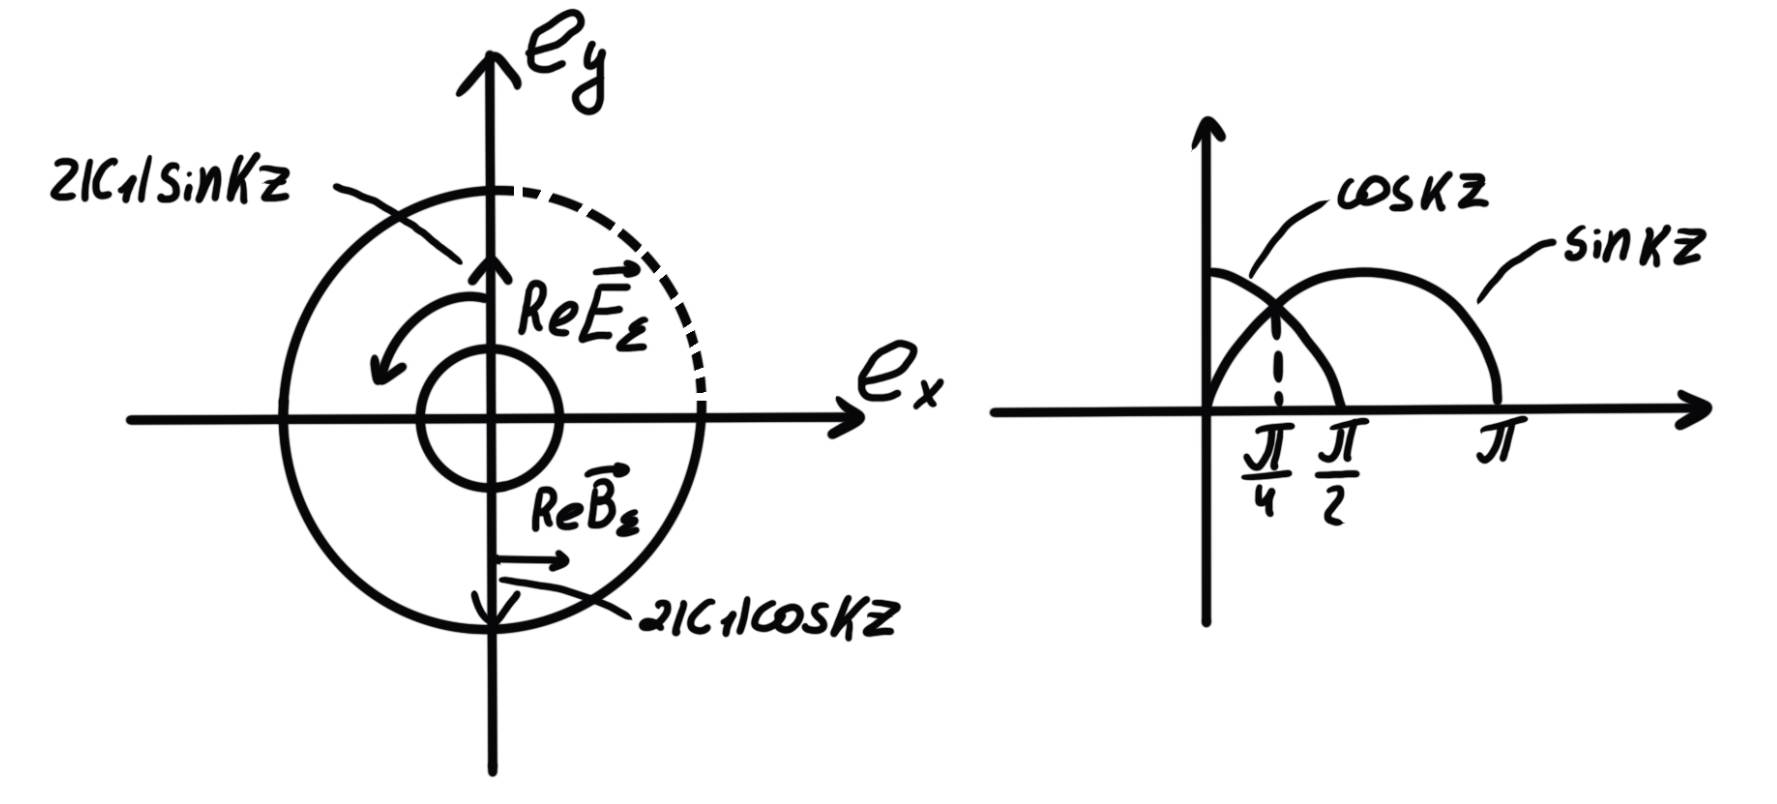
\includegraphics[width=0.6\textwidth]{/Users/vladbelousov/Desktop/Semestr_4-FP-NSU/ЭиО/Лекции_по_дням/image/43.png}
\end{center}

\section{Резонаторы}

- полость, окруженная идеальным проводником. 

В нем накапливаются волны собственной волны резонатора. Таким образом резонатор фильтрует сигнал по определенной частоте и усиливает его сингал. С помощью резонаторов можно ускорять сгустки протонов и электронов.


Способы возбуждения резонаторов: 

1) Штырь с переменным во времени потенциалом. 

2) Петля с переменным током. 

3) Модулированный электронный пучок. 

4) Волновод с бегущей волной. 

Уравнения электромагнитных полей в резонаторе:

\[ \vec{ E } (\vec{r } , t ) = \vec{E_0  }(\vec{r } ) e^{ - i \omega t }   \] 

\[ \vec{B }  (\vec{r } , t )    = \vec{B_0 }(\vec{r } ) e^{ - i \omega t }  \] 

Из уравнений Максвелла следует, что:

\[ \mathrm{rot } \vec{E_0 }(\vec{r } ) e ^{ -i\omega t } = -\frac{i \omega }{c } \vec{B_0 }(\vec{r } ) e^{ -i \omega t}  \Rightarrow \mathrm{div } \vec{B_0 } = 0        \] 

\[ \mathrm{rot } \vec{H_0 }(\vec{r }  ) = - \frac{i \omega }{c } \vec{D_0 }(\vec{r} )  \Rightarrow  \mathrm{div } \vec{D_0  } = 0      \] 

Если внутри резонатора вещество с \( \varepsilon ( \omega ) \) и \( \mu ( \omega ) \Rightarrow \vec{B_0 } = \vec{H_0 } \mu(\omega) ,\text{ }  \vec{D_0 } = \vec{E_0 } \varepsilon ( \omega )   \)   

Граничные условия: 

\[ E_{0 \tau} |_{\text{Г } }  = 0, \quad  B_{0 n} |_{\text{Г } }  = 0  \] 

\begin{center}
    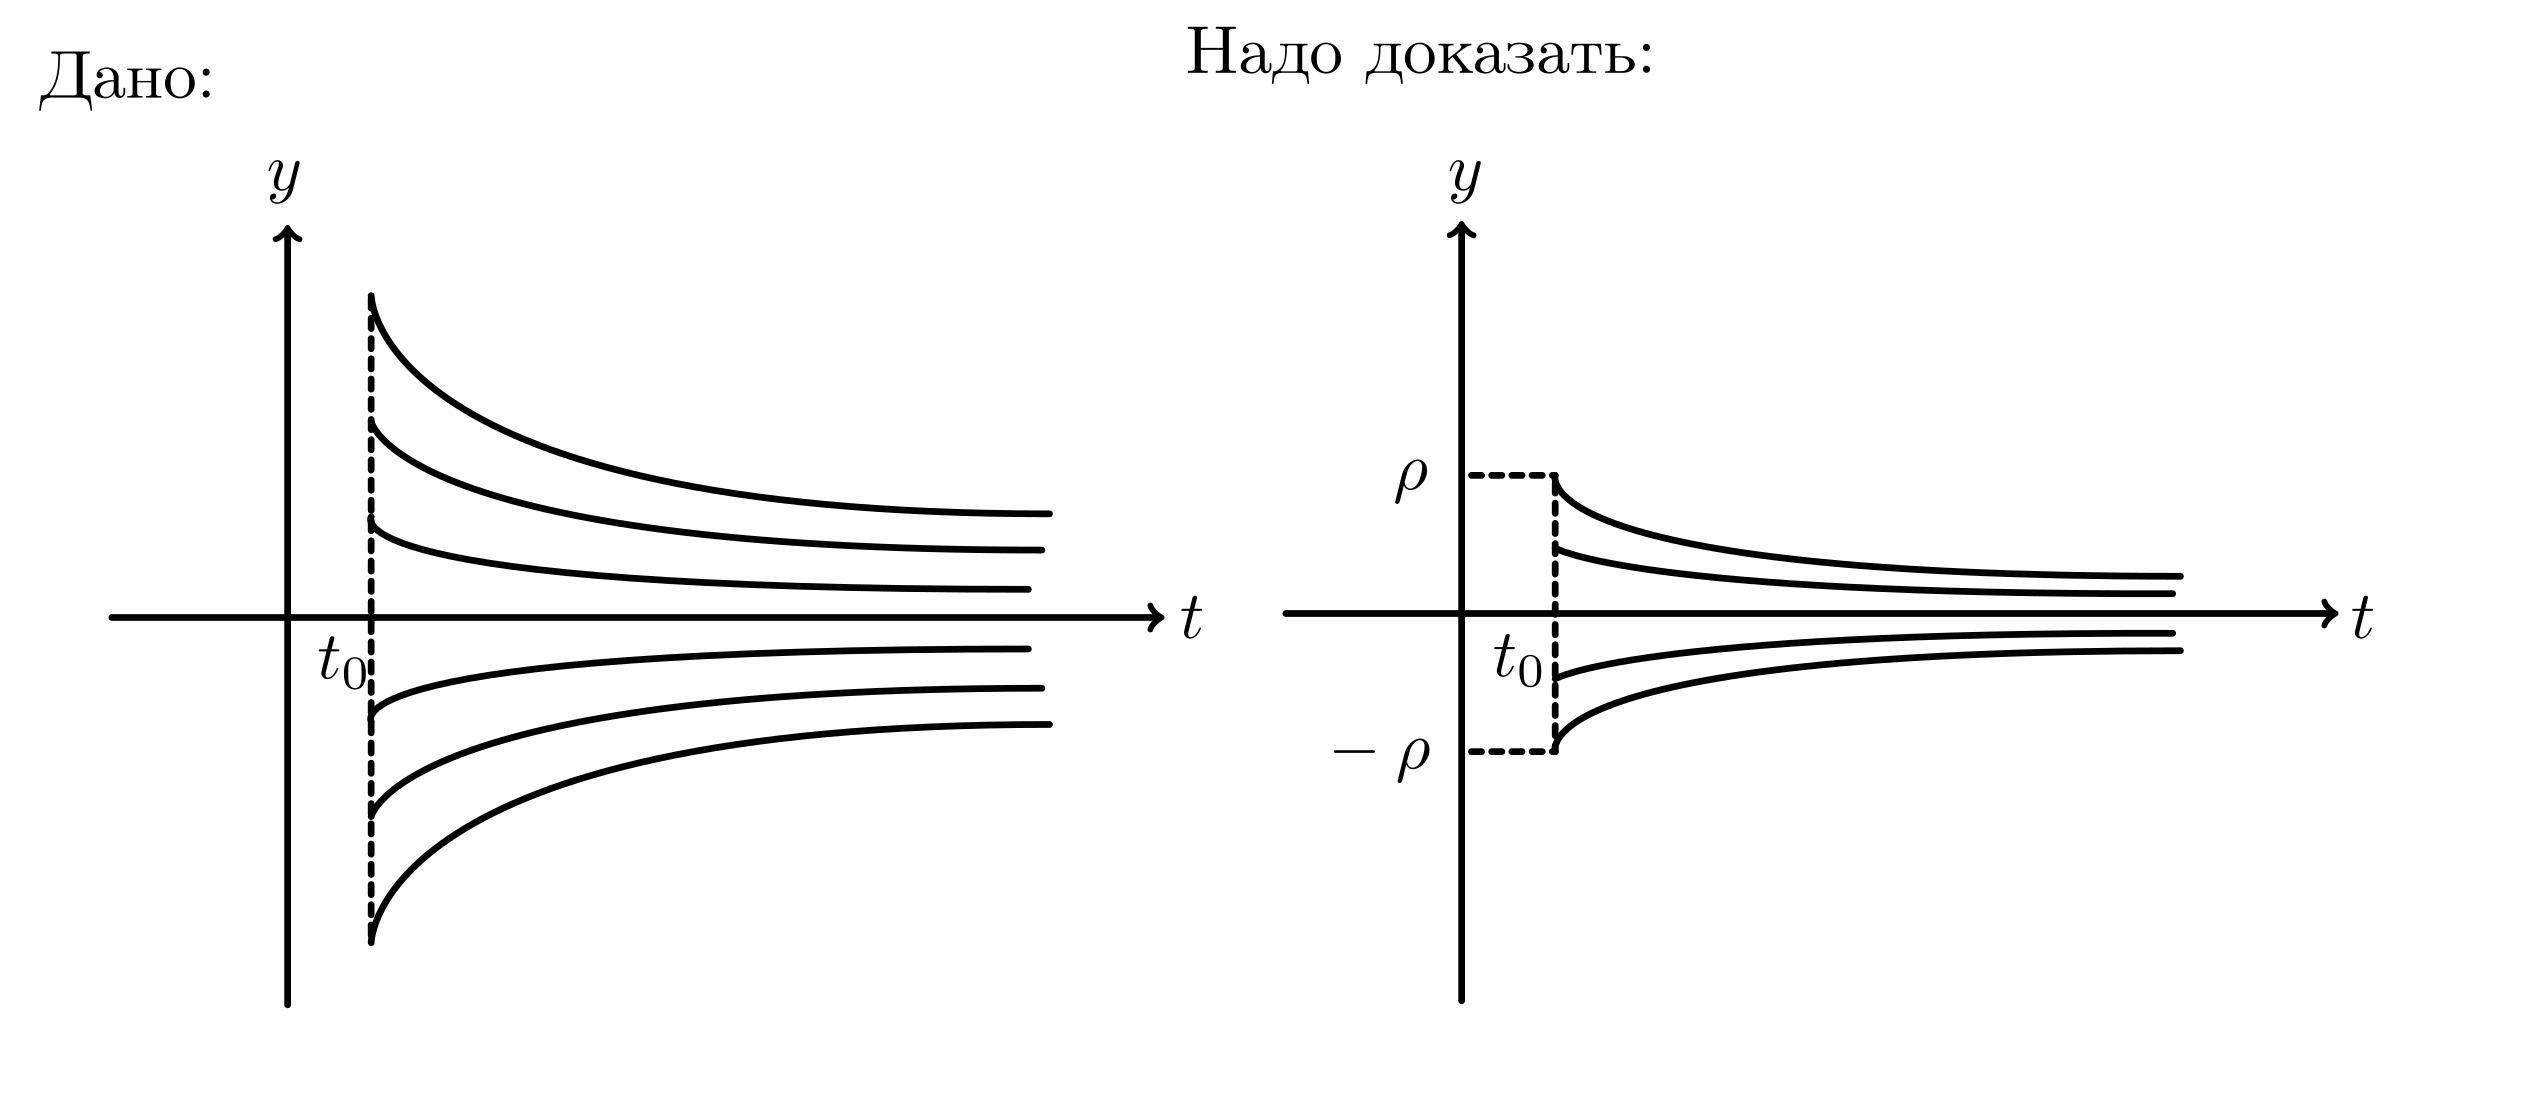
\includegraphics[width=0.2\textwidth]{/Users/vladbelousov/Desktop/Semestr_4-FP-NSU/ЭиО/Лекции_по_дням/image/44.png}
\end{center}

%картинка для пояснения направлений из РУслана 



\[ \begin{aligned}
    \begin{array}{l|}
        \displaystyle (\mathrm{rot }  \vec{E_0})_z =  + \frac{i \omega }{c } B_{0z}   \\
        (\mathrm{rot }  \vec{E_0})_z = \underbrace{\frac{\partial E_{0y } }{\partial  x}}_{=0} - \underbrace{\frac{\partial  E_{0x } }{\partial  y } }_{=0}  \\
        E_{0y } |_{\text{Г} } =0 , \text{ }  E_{0x } |_{\text{Г} } =0 
    \end{array}
    \Rightarrow  B_{0z } = 0
\end{aligned} \] 

Исключим \( \vec{B_0 } (\vec{r } ) \) из уравнений: 

\[ \mathrm{rot } \mathrm{rot } \vec{E_0 }( \vec{r }  ) = \underbrace{\nabla \mathrm{div } \vec{E_0 }(\vec{r } )}_{\frac{\mathrm{div } \vec{D_0 }(\vec{r } )}  {\varepsilon(\omega)} = 0} - \Delta \vec{E_0 } (\vec{r } )  = \frac{i \omega }{c} \mu (\omega )\left( -\frac{ i \omega}{c}  \right) \varepsilon(\omega ) \vec{E_0 }(\vec{r } )   \Rightarrow   \] 

\[  \Rightarrow \begin{aligned}
    \begin{cases}
        \displaystyle \Delta \vec{E_0 }(\vec{r } ) + \frac{ \omega ^2 }{c ^2 }\varepsilon( \omega ) \mu (\omega ) \vec{E_0 }(\vec{r } ) = 0 \\
        \displaystyle \mathrm{div } \vec{E_0 }(\vec{r } ) = 0 
    \end{cases} 
    + \text{Г.У: } E_{0 \tau} |_{\text{Г } }  = 0 
\end{aligned}  \] 

\[ \frac{ \omega ^2 }{c ^2 }\varepsilon( \omega ) \mu (\omega ) = k ^2  \] 

- эта система является краевой трех мерной задачей Штурмана-Лиувиля.

\textbf{Задача Штурма-Лиувиля}: 

1) Решение \( \exists    \)  только для бесконечного ряда чисел \( k_n \) - собственные числа; 

2) Каждому \( k_n \) соответствует как минимум одна собственная функция -  собственное колебание;

3) Набор всех собственных  функций образует фундаментальную систему ортогональных функций, по которым можно разложить поля внешнего источника возбуждения. 

4) \(\displaystyle  \min (k_n ) \sim \frac{1}{l}  \Rightarrow \varepsilon = 1, \text{ }  \mu =1 , \text{ }\omega _{\min  } \sim \frac{c}{l}     \) 

Примеры резонаторов: 

1) Плоский резонатора

\begin{center}
    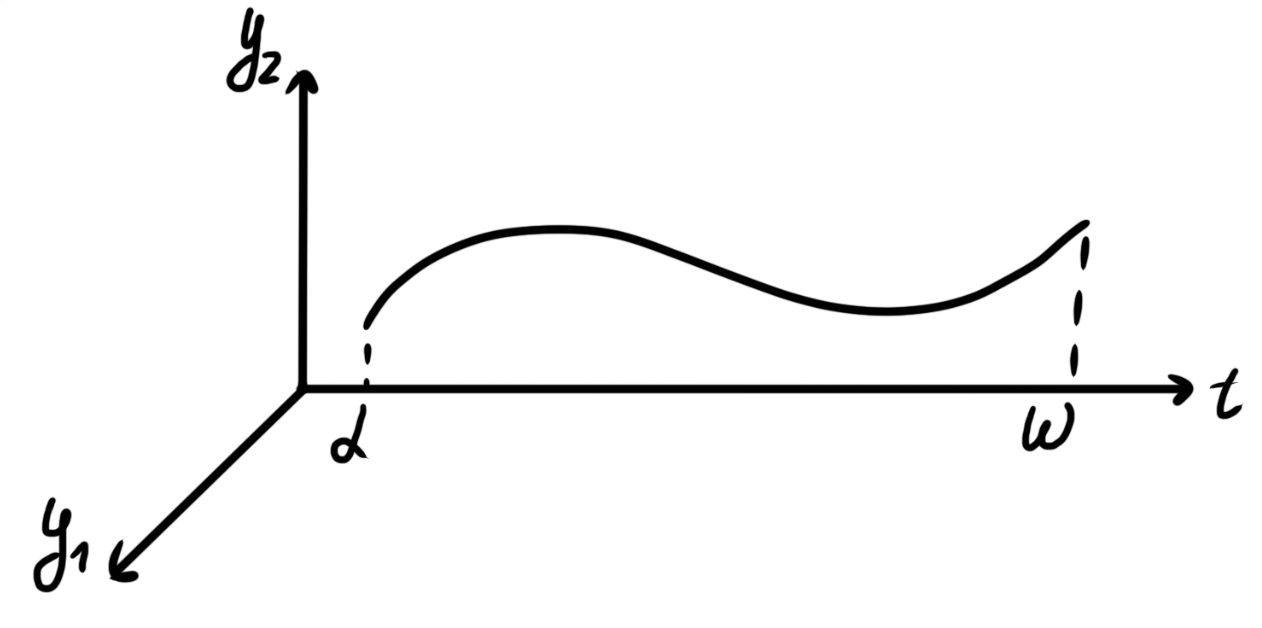
\includegraphics[width=0.3\textwidth]{/Users/vladbelousov/Desktop/Semestr_4-FP-NSU/ЭиО/Лекции_по_дням/image/45.png}
\end{center}

Решение как в задаче про отражение: \( \displaystyle  \vec{E } _{\Sigma} ( \vec{r } , t ) = -2 i \vec{E_0} \sin (kz ) e^{ - i \omega t }  \) 

\[ \Rightarrow \sin (kL ) = 0 \Rightarrow k_m L = m \pi \Rightarrow k_m = \frac{m \pi }{L}   - \text{собственные числа}  \] 

\[ k_{\min  } = \frac{\pi}{ L }  , \text{ } \omega_{ \min } (\varepsilon = 1, \text{ }  \mu =1 )  = \frac{ \pi c }{L}   \] 

\begin{center}
    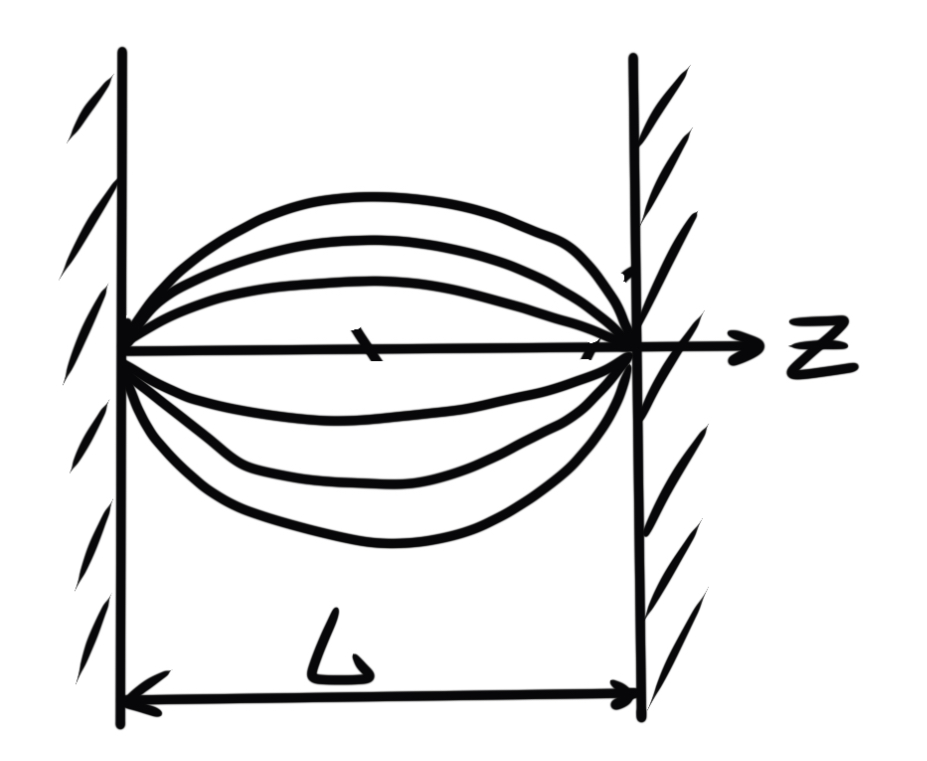
\includegraphics[width=0.3\textwidth]{/Users/vladbelousov/Desktop/Semestr_4-FP-NSU/ЭиО/Лекции_по_дням/image/46.png}
\end{center}

2) Прямоугольный трех мерный резонатор: 

\begin{center}
    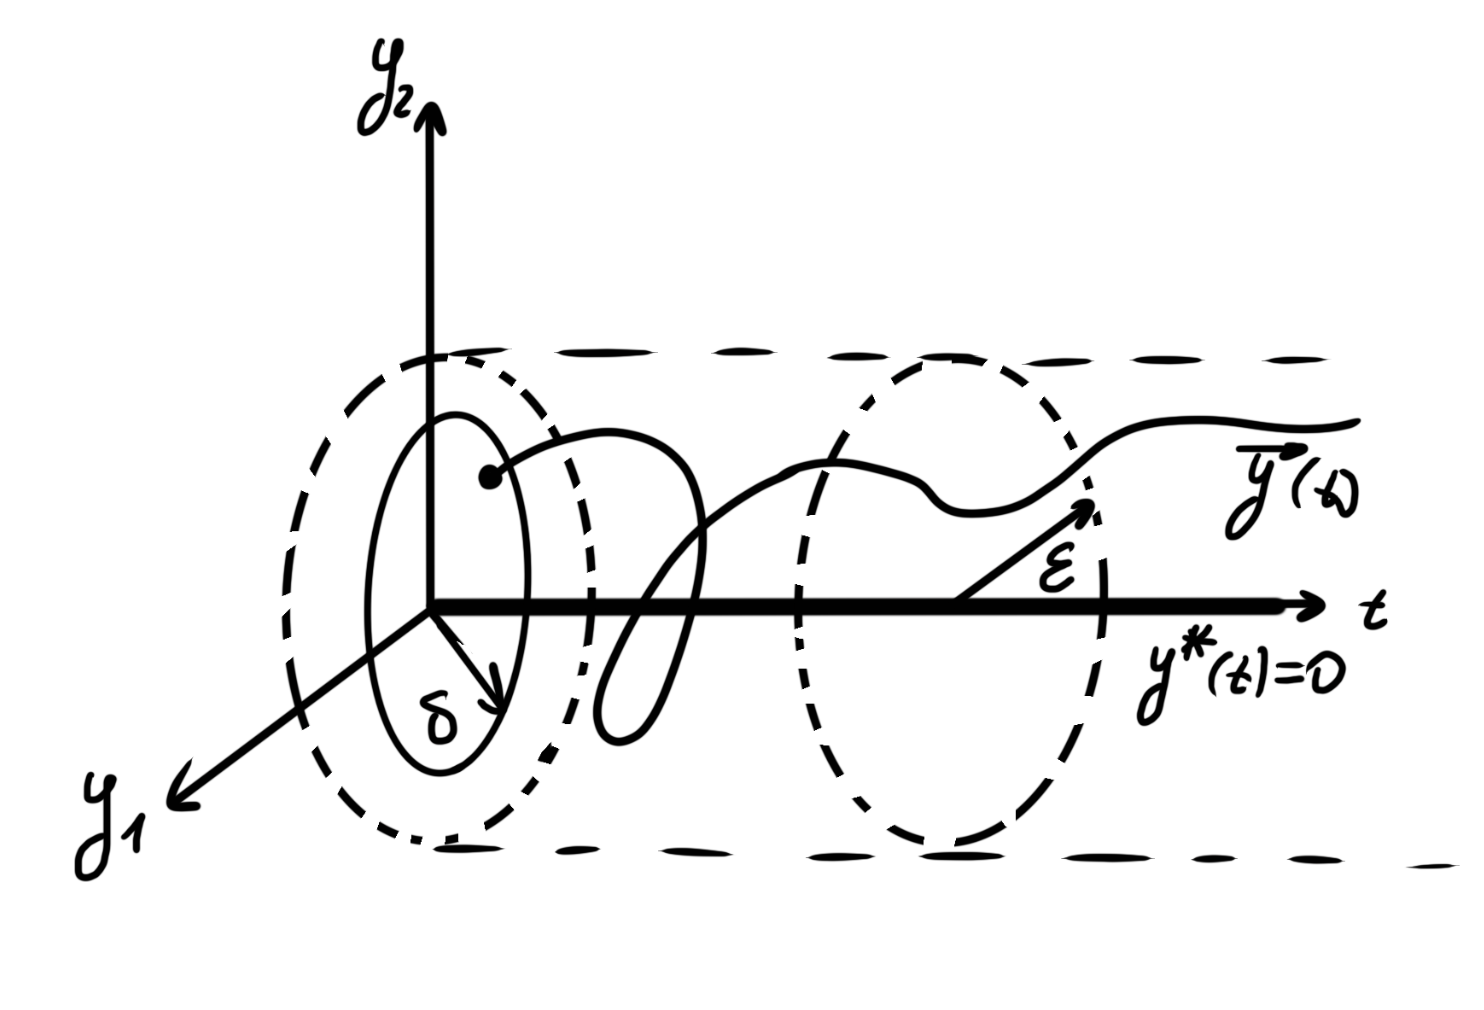
\includegraphics[width=0.4\textwidth]{/Users/vladbelousov/Desktop/Semestr_4-FP-NSU/ЭиО/Лекции_по_дням/image/47.png}
\end{center}

\[ \Delta \vec{E_0 }(\vec{r } )  + k ^2 \vec{E_0 }(\vec{r } ) = 0 , \text{ }  \mathrm{div } \vec{E_0 }(\vec{r } ) = 0 , \text{ } E_{0 \tau} |_{\text{Г } }  = 0   \] 

\[ \left( \frac{\partial  ^2 }{\partial  x ^2 } + \frac{\partial  ^2 }{ \partial  y ^2 } + \frac{\partial  ^2 }{\partial  z ^2 }    \right) \begin{pmatrix}
    E_{0x}\\
    E_{0y} \\
    E_{0z} 
    \end{pmatrix} + k ^2 \begin{pmatrix}
        E_{0x}\\
        E_{0y} \\
        E_{0z} 
    \end{pmatrix} = 0\] 

Пусть \( E_{0x } (\vec{r } )    = E_1 (x) E_2 (y) E_3 (z) \) 

\[ E_2( y )E_3 ( z ) \frac{d ^2 E_1 ( x ) }{dx ^2 } + E_1 ( x ) E_3 ( z ) \frac{d ^2 E_2 ( y ) }{dy ^2 } + E_1 ( x ) E_2 ( y ) \frac{d ^2 E_3 ( z ) }{dz ^2 } + k ^2 E_1 ( x ) E_2 ( y ) E_3 ( z ) = 0 | : E_1 E_2 E_3   \] 

Двигаясь вдоль \( x \)  все члены кроме \( \displaystyle \frac{E_1 ''(x)}{E_1 (x)}  \), точно константы значит используя следующее выражение:  

\[ \frac{E_1 '' ( x )}{E_1(x) } + \frac{E_2 '' ( y )}{E_2(y) } + \frac{E_3 '' ( z )}{E_3(z) } + k ^2 = 0  \text{ , получаем: }  \frac{E_1 ''( x )}{ E_1( x )} = \mathrm{const} ; \underbrace{\text{ } \frac{E_2 ''( y )}{ E_2( y )} = \mathrm{const} , \text{ } \frac{E_3 ''( z )}{ E_3( z )} = \mathrm{const} }_{\text{Аналогочино} }.    \] 

\[ E '' ( x ) = \alpha E (x  ) \quad  \text{ Решение ищем в виде: } E_1(x ) = c_1 e^{\lambda x} \Rightarrow c_1 \lambda ^2 e^{\lambda x } = \alpha c_1e^{\lambda x } \Rightarrow \lambda_{1,2 }  = \pm \sqrt{\alpha }       \] 

\( 1.\text{ }  \alpha > 0 \Rightarrow E (x )  = A e^{ \sqrt{\lambda} x }+ B e^{- \sqrt{\lambda} x }   \) занулить решение на двух стенках \( x=0 , \text{ }  x= a \) -  невозможно 

\( 2.\text{ } \alpha = 0 \Rightarrow E (x ) =  A x + B     \) - аналогично невозможно

\( 3. \text{ }  \alpha < 0 \Rightarrow E ( x )  = A e^{+ i\sqrt{\left\lvert \alpha \right\rvert}x} + B e^{- i\sqrt{\left\lvert \alpha \right\rvert}x}  = c_1 \sin ( \sqrt{\left\lvert \alpha \right\rvert}x + \varphi )  \) - имеет периодически нули, что может удовлетворять границам

Переобозначение: \(\alpha_x = - k ^2 _x , \alpha_y = - k ^2 _y , \alpha_z = - k ^2 _z  \) 

\[ E_{0x}  ( \vec{r } ) = A \sin (k_x x + \alpha_x) \sin (k_y y + \alpha_y) \sin (k_z z + \alpha_z), \alpha_x, \alpha_y, \alpha_z = \mathrm{const} \] 

\[ E_{0y} = B \sin (k_x x + \beta_x) \sin (k_y y + \beta_y) \sin (k_z z + \beta_z), \beta_x, \beta_y, \beta_z = \mathrm{const}  \] 

\[ E_{0z} = D \sin (k_x x + \gamma_x) \sin (k_y y + \gamma_y) \sin (k_z z + \gamma_z), \gamma_x, \gamma_y, \gamma_z = \mathrm{const} \] 

Граничные условия: \( x= 0 \Rightarrow E_y = 0 , \text{ }  E_z = 0  \text{ при } \forall y,z \Rightarrow \beta_x = 0 , \gamma_x = 0   \)  

    \[ x = a \Rightarrow E_{0y }  =0, \text{ }  E_{0z } = 0 \text{ при }  \forall  y ,z  \Rightarrow k_x a = n_x \pi \Rightarrow k_x = \frac{ n_x \pi } {a } , \text{ }  n_x \in  \mathbb{Z}    \] 

    \[ y = 0 \Rightarrow E_{0x } = 0, \text{ }  E_{0z } = 0 \text{ при } \forall x,z \Rightarrow \alpha_y = \gamma _y = 0  \] 

    \[ y = b \Rightarrow E_{0x } = 0, \text{ }  E_{0z } = 0 \text{ при } \forall x,z \Rightarrow k_y b = n_y \pi \Rightarrow k_y = \frac{ n_y \pi } {b } , \text{ }  n_y \in  \mathbb{Z}    \] 

    \[ z= 0 \Rightarrow E_{0x } = 0, \text{ }  E_{0y } = 0 \text{ при } \forall x,y \Rightarrow \alpha_z = \beta _z = 0  \] 

    \[ z= d \Rightarrow E_{0x } = 0, \text{ }  E_{0y } = 0 \text{ при } \forall x,y \Rightarrow k_z d = n_z \pi \Rightarrow k_z = \frac{ n_z \pi } {dч } , \text{ }  n_z \in  \mathbb{Z}    \] 

    \[ \mathrm{div } \vec{E_0} = \frac{\partial  }{\partial  x } E_{0x} + \frac{\partial  }{\partial  y } E_{0y } + \frac{\partial  }{\partial  z }E _{0z } =       \] 

    \[ =\sin (k_x x) \sin (k_y y )\sin (k_z z) \bigg[ \underbrace{\frac{k_xA \cos (k_x x + \alpha_x) }{\sin (k_x x)}}_{\mathrm{const} }+ \underbrace{\frac{k_yB \cos (k_y y + \beta_y) }{\sin (k_y y)}}_{\mathrm{const}} + \underbrace{\frac{k_z D  \cos (k_z  z+ \gamma_z) }{\sin (k_z  z)}}_{\mathrm{const}}  \bigg]  = 0       \] 


    \( \text{ при } \forall  x, y , z \) 

    \[ \Rightarrow \alpha_x = \frac{\pi}{2 }  , \beta_y = \frac{\pi}{2 } , \gamma_z = \frac{\pi}{2 } \Rightarrow k_x A + k_y B + k_z D = 0 \text{  или }   (\vec{k } , (\overrightarrow{A,B,C}) ) = 0  \] 

    Конечный ответ: 

    \[ \begin{aligned}
        E_{0x }  (\vec{r } ) &= A \cos (k_x x )\sin (k_y y )\sin (k_z z) \\
        E_{0y}(\vec{r} ) &= B \sin (k_x x )\cos (k_y y )\sin (k_z z)  \quad  \oplus \quad k_x A + k_y B + k_z D = 0 + \text{ Г.У. } \vec{E} _{0 \tau } |_{\text{Г} } = 0      \\
        E_{0z}(\vec{r} ) &= D \sin (k_x x )\sin (k_y y )\cos (k_z z) 
    \end{aligned} \] 


%%-------------------------------%%

% Закрытие документа, если файл компилируется отдельно
\ifdefined\mainfile
    % Если это основной файл, не нужно заканчивать документ
\else
    \end{document}
\fi